\documentclass[tikz,border=10pt]{standalone}
\usepackage{amsmath}
\usetikzlibrary{arrows.meta, positioning, calc, decorations.pathreplacing}
\definecolor{c1}{HTML}{000000}
\definecolor{c2}{HTML}{233D4D}
\definecolor{c3}{HTML}{FE7F2D}
\definecolor{c4}{HTML}{EAECF0}
\definecolor{labelcolor}{HTML}{5F6B75}
\begin{document}
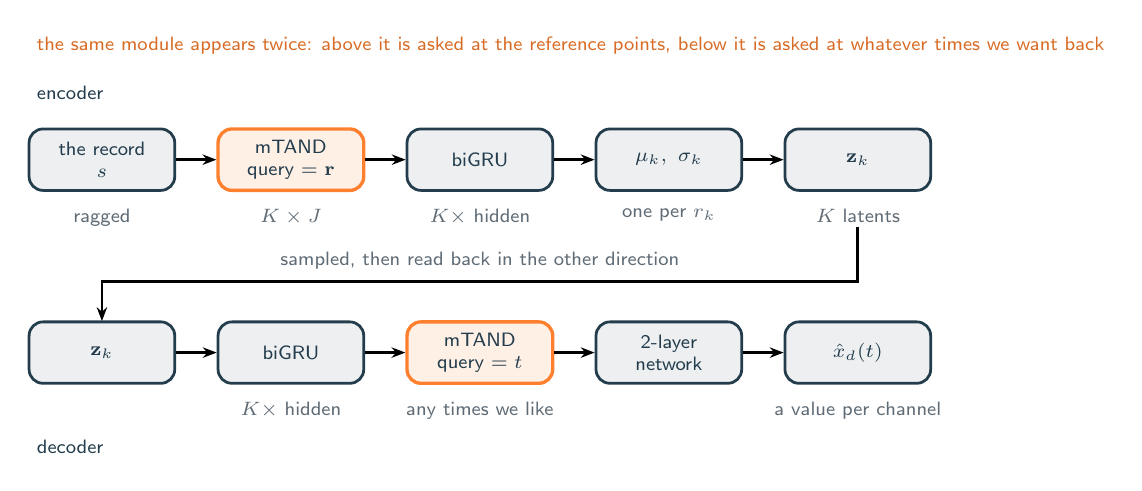
\begin{tikzpicture}[
    every node/.style={font=\sffamily},
    lab/.style={font=\sffamily\scriptsize, text=labelcolor},
    tag/.style={font=\sffamily\scriptsize, text=c2},
    hot/.style={font=\sffamily\scriptsize, text=c3!85!black},
    blk/.style={rectangle, rounded corners=5pt, draw=c2, fill=c2!8, text=c2,
                line width=1.0pt, minimum width=1.85cm, minimum height=0.78cm,
                align=center, font=\sffamily\scriptsize},
    mod/.style={rectangle, rounded corners=5pt, draw=c3, fill=c3!12, text=c2,
                line width=1.2pt, minimum width=1.85cm, minimum height=0.78cm,
                align=center, font=\sffamily\scriptsize},
    arr/.style={-{Stealth[length=5pt]}, line width=1.0pt, color=c1},
]

% ================================================================ encoder
\node[tag, anchor=west] at (0.30, 5.55) {encoder};
\node[blk] (s)  at (1.25, 4.70) {the record\\ $s$};
\node[mod] (me) at (3.65, 4.70) {mTAND\\ query $=\mathbf{r}$};
\node[blk] (ge) at (6.05, 4.70) {biGRU};
\node[blk] (mu) at (8.45, 4.70) {$\mu_k,\ \sigma_k$};
\node[blk] (z1) at (10.85, 4.70) {$\mathbf{z}_k$};
\foreach \a/\b in {s/me, me/ge, ge/mu, mu/z1}{ \draw[arr] (\a) -- (\b); }
\node[lab, anchor=north] at (1.25, 4.20) {ragged};
\node[lab, anchor=north] at (3.65, 4.20) {$K \times J$};
\node[lab, anchor=north] at (6.05, 4.20) {$K \times$ hidden};
\node[lab, anchor=north] at (8.45, 4.20) {one per $r_k$};
\node[lab, anchor=north] at (10.85, 4.20) {$K$ latents};

% the latent is handed down
\draw[arr] (10.85, 3.85) -- (10.85, 3.15) -- (1.25, 3.15) -- (1.25, 2.65);
\node[lab, anchor=south] at (6.05, 3.18) {sampled, then read back in the other direction};

% ================================================================ decoder
\node[tag, anchor=west] at (0.30, 1.05) {decoder};
\node[blk] (z2) at (1.25, 2.25) {$\mathbf{z}_k$};
\node[blk] (gd) at (3.65, 2.25) {biGRU};
\node[mod] (md) at (6.05, 2.25) {mTAND\\ query $= t$};
\node[blk] (fc) at (8.45, 2.25) {2-layer\\ network};
\node[blk] (xh) at (10.85, 2.25) {$\hat{x}_d(t)$};
\foreach \a/\b in {z2/gd, gd/md, md/fc, fc/xh}{ \draw[arr] (\a) -- (\b); }
\node[lab, anchor=north] at (3.65, 1.75) {$K \times$ hidden};
\node[lab, anchor=north] at (6.05, 1.75) {any times we like};
\node[lab, anchor=north] at (10.85, 1.75) {a value per channel};

% the swap
\node[hot, anchor=west, align=left] at (0.30, 6.15)
    {the same module appears twice: above it is asked at the reference points,
     below it is asked at whatever times we want back};
\end{tikzpicture}
\end{document}
